\documentclass[10 pt,usenames,dvipsnames, oneside]{article}
\usepackage{../../../modelo-ensino-medio}



\begin{document}

\begin{center}
  \begin{minipage}[l]{3cm}

\includegraphics[width=2cm]{logo}    
\end{minipage}\hfill
\begin{minipage}[r]{.8\textwidth}
 {\Large \scshape Atividade: Brasil e Reino Unido na pandemia}  
\end{minipage}
\end{center}
\vspace{.2cm}

\ifdefined\prof
%Habilidades da BNCC
\begin{objetivos}
\item \textbf{EM13MAT403} Analisar e estabelecer relações, com ou sem apoio de tecnologias digitais, entre as representações de funções exponencial e logarítmica expressas em tabelas e em plano cartesiano, para identificar as características fundamentais (domínio, imagem, crescimento) de cada função.
\item \textbf{EM13MAT101} Interpretar criticamente situações econômicas, sociais e fatos relativos às Ciências da Natureza que envolvam a variação de grandezas, pela análise dos gráficos das funções representadas e das taxas de variação, com ou sem apoio de tecnologias digitais.

\item \textbf{EM13MAT102} Analisar tabelas, gráficos e amostras de pesquisas estatísticas apresentadas em relatórios divulgados por diferentes meios de comunicação, identificando, quando for o caso, inadequações que possam induzir a erros de interpretação, como escalas e amostras não apropriadas.
\end{objetivos}

%Caixa do Para o Professor
\begin{goals}
%Objetivos específicos
\begin{enumerate}
\item Utilizar o ajuste de curvas para identificar tendências em dados reais.
\item Interpretar criticamente a situação dos dois países na pandemia de Covid-19 pela análise dos gráficos das funções representadas e das taxas de variação, com ou sem apoio de tecnologias digitais.
\item Analisar tabelas, gráficos e amostras de pesquisas estatísticas apresentadas em relatórios divulgados por diferentes meios de comunicação, identificando, quando for o caso, inadequações que possam induzir a erros de interpretação, como escalas e amostras não apropriadas.
\end{enumerate}

\tcblower

%Orientações e sugestões
\begin{itemize}
\item A atividade propõem a análise de tendências nos gráficos apresentados comparando as situações do Brasil e do Reino Unido. O resultado esperado da atividade não é uma resposta exata, mas uma discussão sobre o tema, que pode ser realizada em grupo na sala de aula. Espera-se que os alunos identifiquem uma mudança na tendência do gráfico do Reino Unido, de crescimento exponencial (muito rápido) para logarítmico (mais lento) um pouco depois do dia 10 de abril, enquanto que no Brasil o número de mortos parece estar abandonando o crescimento exponencial somente em 13 de junho. O número de mortos no Brasil, no momento da aparente mudança no perfil, está entre 3x e 4x o número de mortos no Reino Unido no momento de mudança. Isso poderia sugerir que o Brasil atingiria entre 3x e 4x o número de mortos, se a pandemia continuasse se  desenvolvendo da mesma forma nos dois países e o perfil final dos dois países fosse parecido (o que não sabemos antes do final da pandemia). Recomenda-se que o/a professor/a busque dados atualizados da pandemia e mostre aos estudantes, assim os alunos poderiam verificar se as suas hipóteses e previsões realizadas concretizaram-se.

	Ainda na atividade é importante ressaltar em uma análise que há grandes diferenças entre os países e essas contribuem bastante para o resultado final. Essa atividade poderia ser desenvolvida de forma interdisciplinar com a disciplina de geografia, que poderia explorar diferenças demográficas, sociais, dos sistemas de saúde, socio-econômicas e das reações socio-políticas dos países. Por exemplo, citamos o fato óbvio que as populações do Brasil (de 209,5 milhões (2018), segundo o Banco mundial) e do Reino Unido (de 66,65 milhões (2018), segundo o Banco Mundial) são fatores importantes a se levar em consideração.
\end{itemize}
\end{goals}

\bigskip
\begin{center}
{\large \scshape Atividade}
\end{center}
\fi

Observando o gráfico abaixo, em que data (aproximadamente) o crescimento mudou de exponencial para logarítmico no Reino Unido? E no Brasil? Apesar do número ser parecido na data final do gráfico, você acredita que o número total de mortos manteve-se próximo? Que fatores sociais, econômicos e demográficos podem ter influenciado o desenvolvimento da pandemia nesses países? 

\begin{figure}[H]
\centering
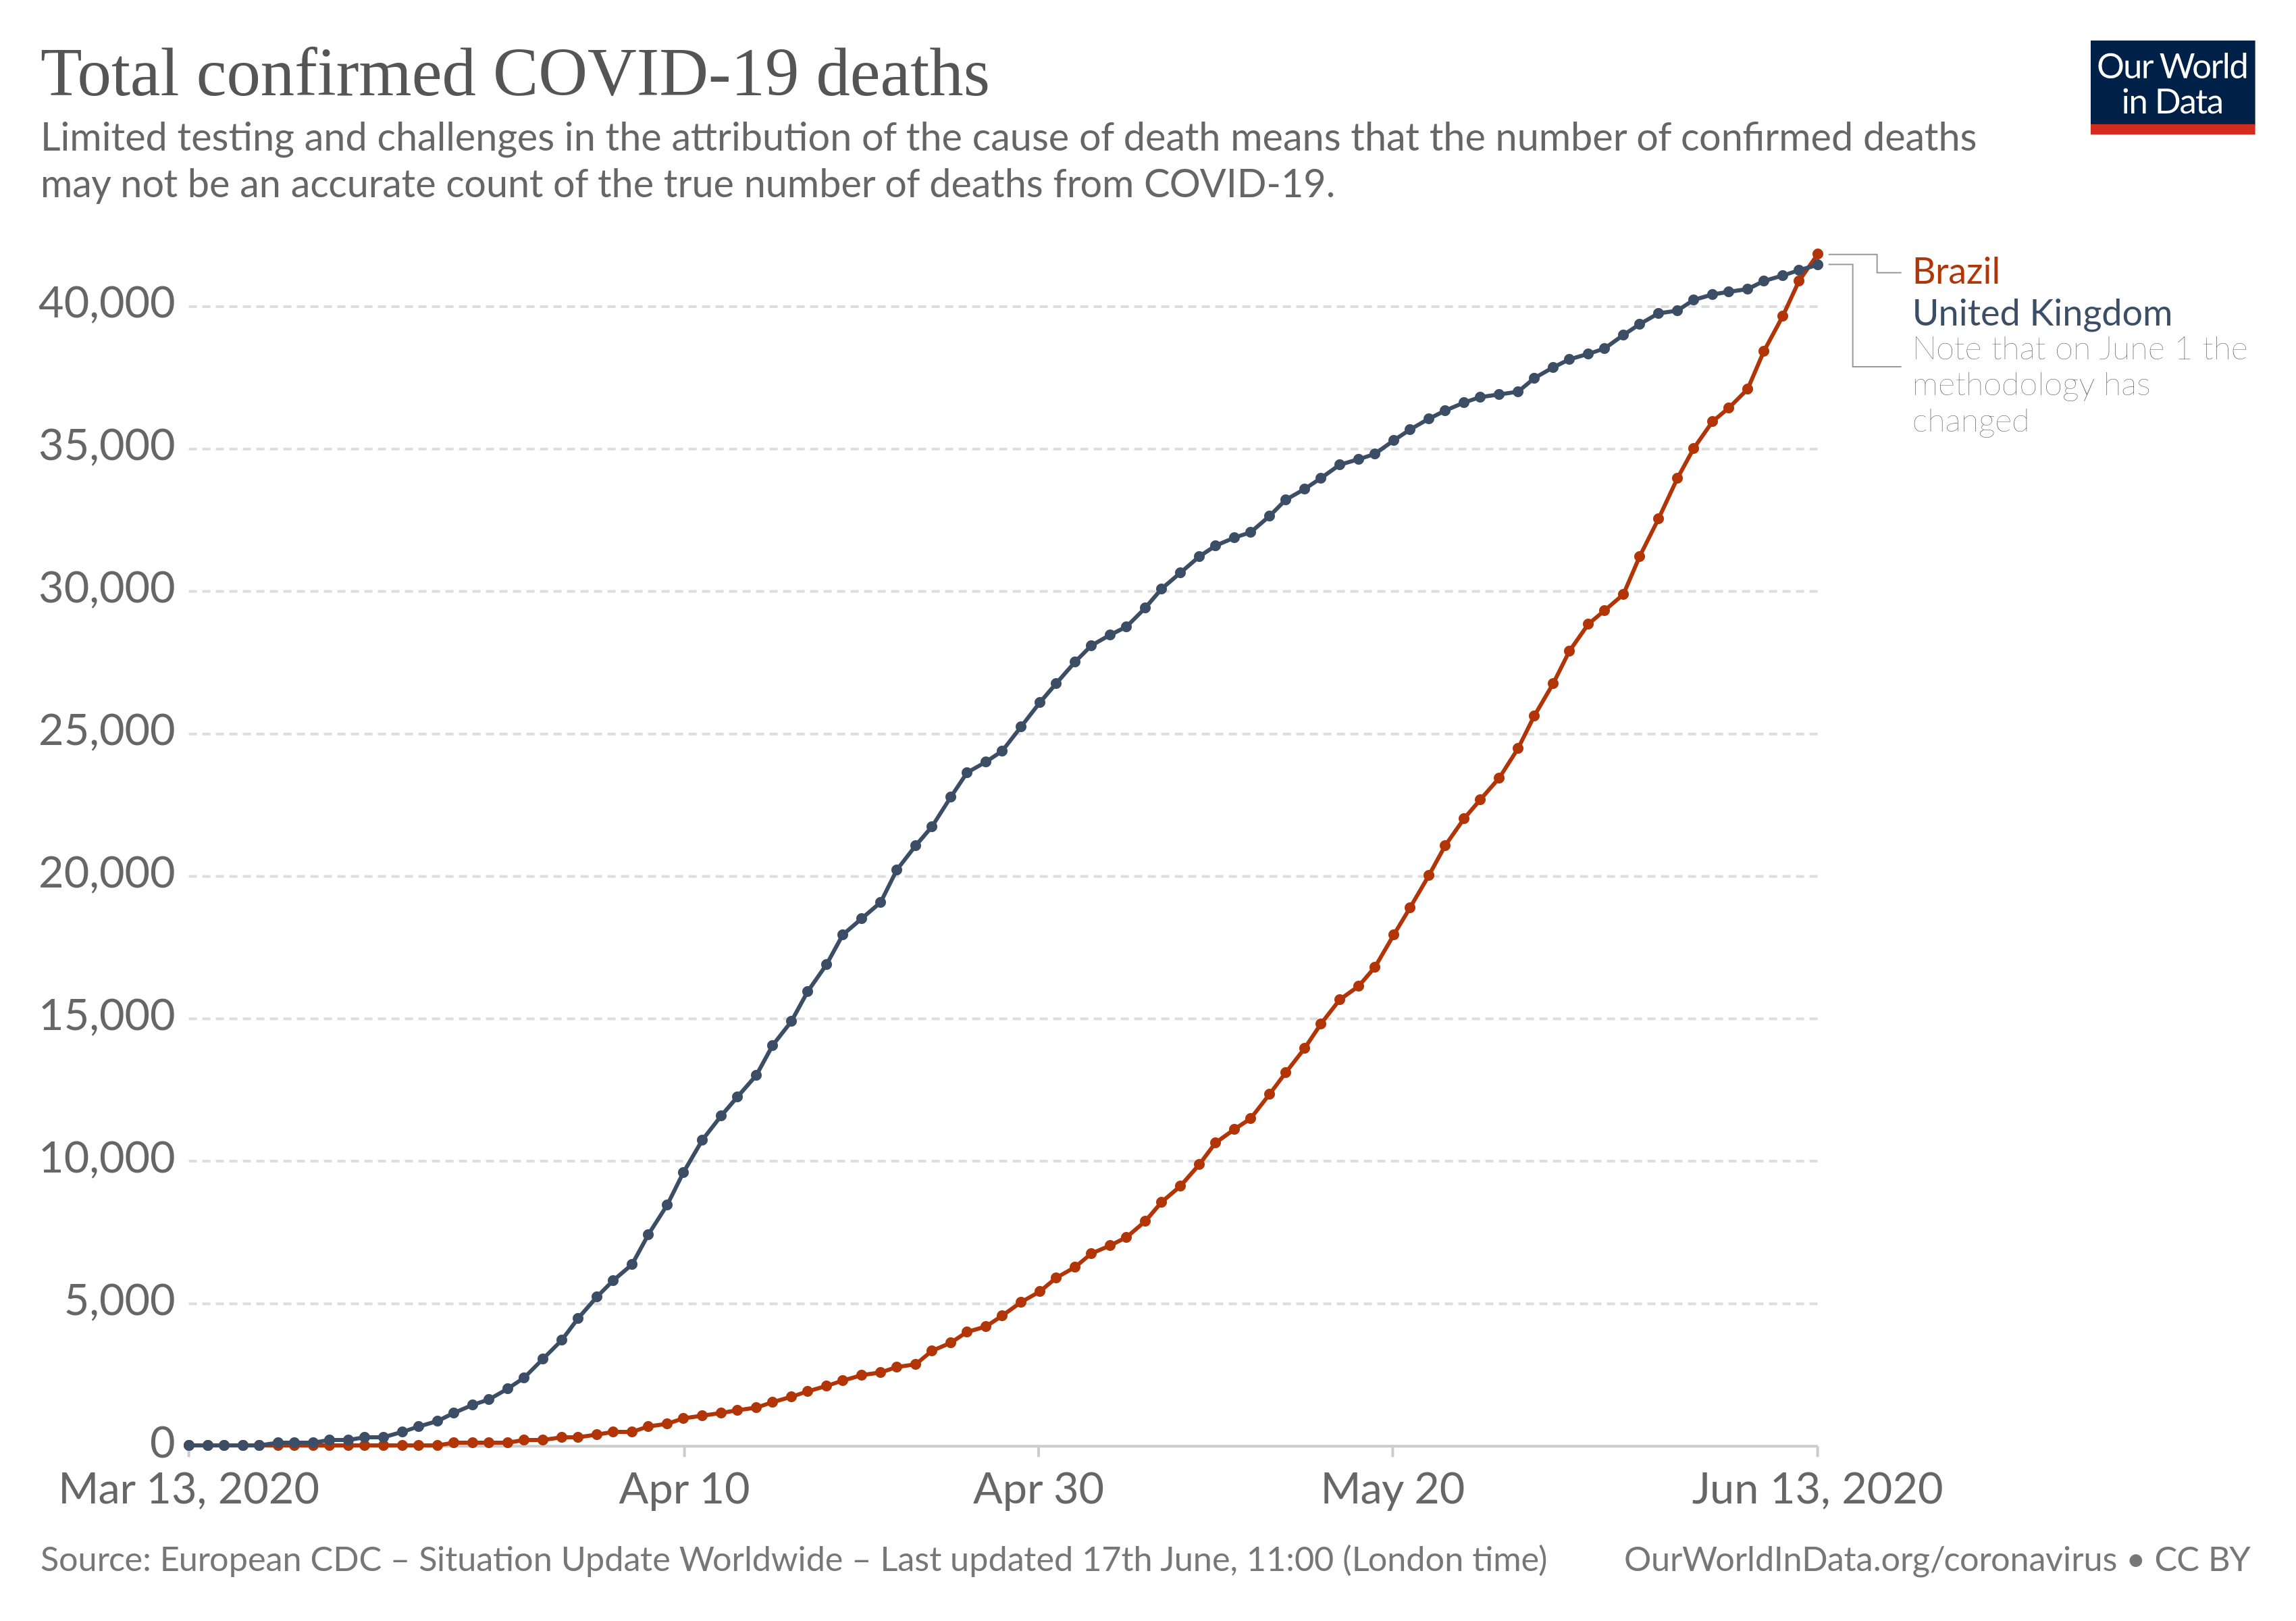
\includegraphics[width=0.8\linewidth]{Brasil_Inglaterra_mortes.png}

\caption{Mortes confirmadas Covid-19 no Brasil e no Reino Unido. \\ Fonte: \textit{Our World in Data} (\url{ourworldindata.org}}
\end{figure}

\ifdefined\prof
% \begin{solucao}

% \begin{enumerate}
% \item
% \end{enumerate}

% \end{solucao}
\fi

\end{document}